\documentclass{beamer}
\usetheme{metropolis}
\usecolortheme{seahorse}

% ---- Packages (XeLaTeX 권장) ----
\usepackage{graphicx}
\usepackage{kotex}        % 한글
\usepackage{ragged2e}
\usepackage{tikz}
\usepackage{amsmath,amssymb}
\usetikzlibrary{arrows.meta,positioning}
\usepackage{mismath}
\usepackage{animate} 
%\usepackage{authblk}
% ---- (beamer가 hyperref를 로드하므로 별도 \usepackage{hyperref} 불필요) ----

% ---- Optional: 섹션 페이지 스타일 ----
\setbeamerfont{section page number}{size=\Huge,series=\bfseries}
\setbeamerfont{section page title}{size=\Huge,series=\bfseries}
\setbeamerfont{section page subtitle}{size=\large,series=\mdseries}
\setbeamercolor{section page number}{fg=structure!80!black}
\setbeamercolor{section page title}{fg=structure}
\setbeamercolor{section page subtitle}{fg=black!70}
\setbeamercolor{title separator}{fg=black!70}
\setbeamercolor{block title}{bg=black!20,fg=black}
\setbeamercolor{block body}{bg=black!10,fg=black}
\setbeamertemplate{section page}{
  \begin{centering}
    \begin{beamercolorbox}[sep=12pt,center,shadow=true,rounded=true]{section title}
      \usebeamerfont{section title}\insertsection\par
    \end{beamercolorbox}
  \end{centering}
}

\title{Deep Learning 1}
\subtitle{Introduction to Machine Learning}
\author{안성민\\ 김영주}
\date{\today}

\begin{document}

\maketitle

\begin{frame}{목차}
  \tableofcontents
\end{frame}

\section{Introduction}
\begin{frame}{Machine Learning}
    1. 컴퓨터가 스스로 학습하는 알고리즘이다.\\
    2. 이 알고리즘의 산물을 AI 모델이라 한다.\\
    3. 머신 러닝 줄여서 ML\\
    \begin{figure}
        \centering
        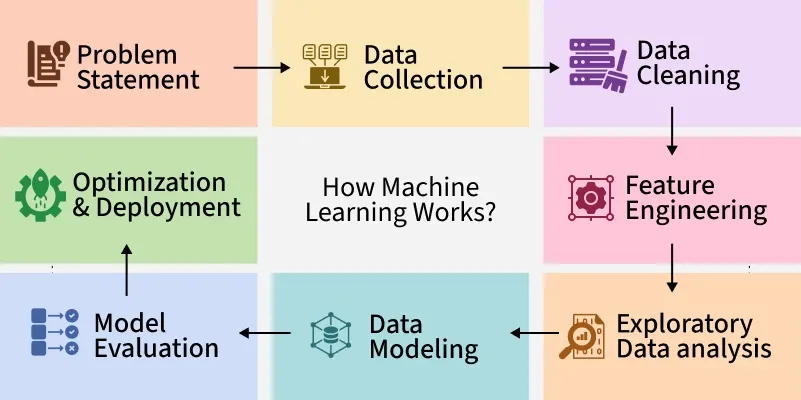
\includegraphics[width=0.5\linewidth]{Images/Machine Learning.png}
        \caption{머신 러닝 개요}
        \label{fig:ML}
    \end{figure}
\end{frame}
\begin{frame}{기초 ML}
    1. 선형근사 같은 간단한 형태는 이미 최적해가 구해져 있다\\
    2. 복잡한 계산이 아닌 간단한 대입으로 끝난다.\\
    3. 이로 인해 ML은 시간이 오래 걸리지 않는다.
    
\end{frame}
\begin{frame}{Feature \& Sample}
    1. 입력으로 넣어주는 변수를 feature\\
    2. 데이터 1개를 Sample이라 한다. 
\end{frame}

\begin{frame}{Deep Learning}
    1. 머신 러닝의 한 분파로, 가장 인기가 많다\\
    2. 높은 성능과 좋은 결과가 나온다.\\
    3. 학습과 추론에 엄청난 연산량이 요구된다.
    \begin{figure}
        \centering
        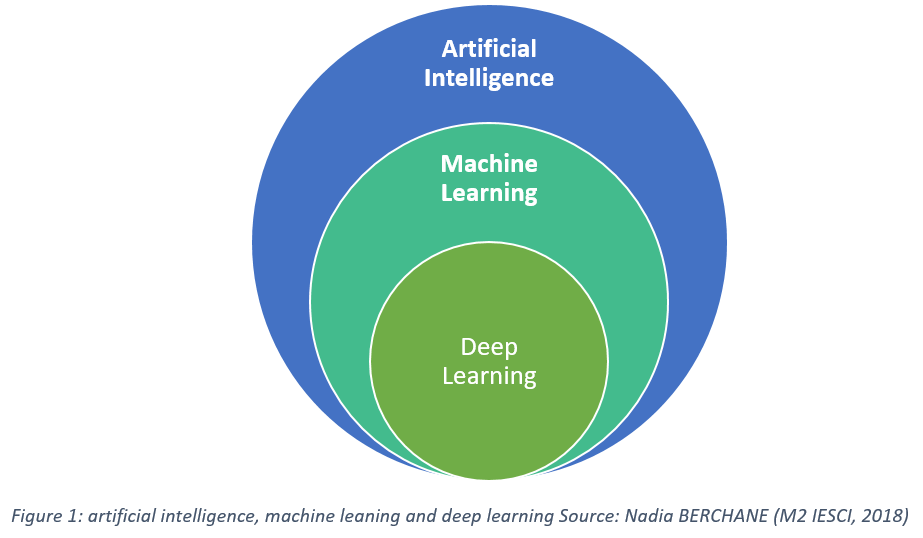
\includegraphics[width=0.5\linewidth]{Images/AI.png}
        \caption{AI 개요}
        \label{fig:AI}
    \end{figure}
\end{frame}
\section{Optimization}
\begin{frame}{Optimization}
    1. AI 학습에 근간이 되는 것이 최적화(optimization)이다.\\
    2. AI는 어떤 수식이다.\\
    3. AI 훈련은 수식의 계수를 최적화 기법을 이용해서 잘 설정\\ 높은 정확도를 가지게 하는 것\\
    4. 이러한 계수를 파라미터/가중치라 한다.
\end{frame}

\begin{frame}{Gradient Descent}
    1. 경사 하강법(gradient Descent, 줄여서 GD)라 한다.\\
    2. 최적화 알고리즘의 가장 기본적인 형태이다. \\
    3. 목적함수 $f(x)$에 대해,\\
    $x_{n+1}=x_{n}-\alpha\nabla f(x_{n})$\\
    처럼 계수 x를 바꿔서 함수 f의 값을 최소화 한다.\\
    \begin{figure}
        \centering
        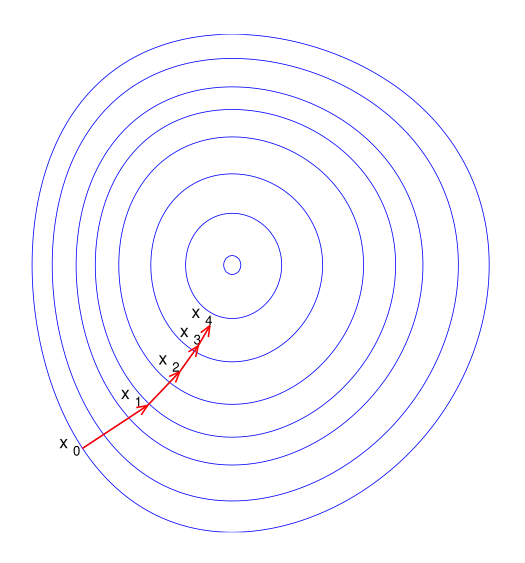
\includegraphics[width=0.3\linewidth]{Images/gradient.png}
        \caption{경사 하강법}
        \label{fig:gradient descent}
    \end{figure}
\end{frame}
\begin{frame}{Gradeint Descent 2}
    1. 한계: 복잡한 문제에 대한 최적화가 어렵다\\
    2. 국소 최적해(local optimum)에 빠지기 쉽다\\
    3. 이를 해결하기 위해 여러 가지 최적화 기법이 나오지만 완전한 해답이 되지 못했다.\\
    
\begin{figure}
    \centering
    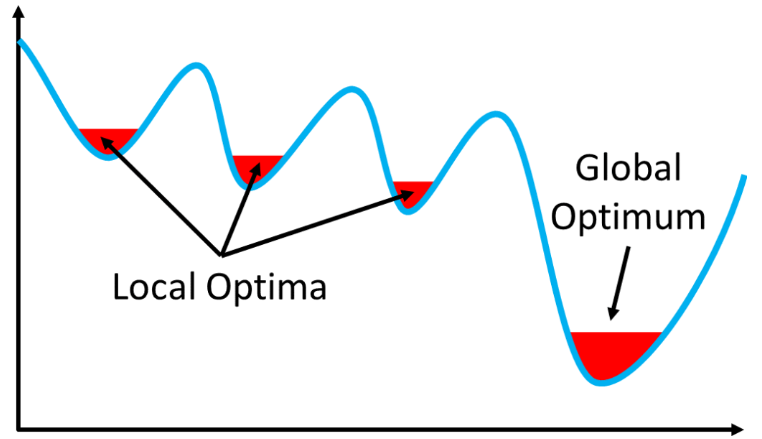
\includegraphics[width=0.5\linewidth]{Images/local.png}
    \caption{local/global optimum}
    \label{fig:local/global optimum}
\end{figure}
\end{frame}
\begin{frame}{ADAM \& LION}
    1. ADAM:\\
    Open AI에서 만든 최적화 기법\\
    Gradient Descent의 발전된 형태\\
    세계관 최강자\\
\begin{figure}[t]
  \centering
  % 10 fps (GIF이 frame당 100ms였음)
  \animategraphics[
    autoplay,loop,
    poster=first,
    width=0.5\linewidth
  ]{10}{optimizer_frames/opt_}{0001}{0090}
  \caption{Optimizer Comparison}
  \label{fig:optimizer-comparison}
\end{figure}

\end{frame}
\begin{frame}{ADAM \& LION}
    2. LION:\\
    구글에서 개발한 최적화 기법\\
    ADAM과 유사 또는 그 이상의 성능을 가짐\\
\end{frame}
\section{Math}
\begin{frame}{Numbers}
    1. 딥러닝의 대부분은 행렬곱으로 이루어진다\\
    2. 차원에 따른 수의 명명\\
    2.1 0차원: 스칼라\\
    2.2 1차원: 벡터\\
    2.3 2차원:행렬\\
    2.4 3차원+: 텐서
\end{frame}
\begin{frame}{Calculation: Vector}
    1. 덧셈 뺑셈은 물리와 유사\\
    2. 곱은 주로 내적을 사용함\\
    3. 이 식은 다중 선형 회귀를 벡터 연산으로 표현
    \begin{equation*}
        y = 
        \begin{bmatrix}
        x_1 & x_2 & x_3 & \cdots & x_n
        \end{bmatrix}
        \begin{bmatrix}
        w_1 \\
        w_2 \\
        w_3 \\
        \vdots \\
        w_n
        \end{bmatrix}
        + b 
        = x_1 w_1 + x_2 w_2 + \cdots + x_n w_n + b
    \end{equation*}
\end{frame}
\begin{frame}{Calculation: Matrix}
    1. 벡터 처럼 행렬로도 나타낼 수 있다.\\
    2. $H(X)=WX+B$, 행렬곱을 위한 기본 조건을 만족해야 함.\\
    3. 딥러닝이 이와 비슷하게 진행된다.
    \begin{equation*}
        \begin{bmatrix}
        w_1 \\ 
        w_2 \\ 
        w_3 \\ 
        w_4
        \end{bmatrix}
        \begin{bmatrix}
        x_{11} & x_{12} & x_{13} & x_{14} \\
        x_{21} & x_{22} & x_{23} & x_{24}\\
        x_{31} & x_{32} & x_{33} & x_{34}\\
        x_{41} & x_{42} & x_{43} & x_{44}\\
        x_{51} & x_{52} & x_{53} & x_{54}\\

        \end{bmatrix}
        + 
        \begin{bmatrix}
        b \\ 
        b \\ 
        b \\ 
        b \\ 
        b
        \end{bmatrix}
        =
        \begin{bmatrix}
        y_1 \\ 
        y_2 \\ 
        y_3 \\ 
        y_4 \\ 
        y_5
        \end{bmatrix}
    \end{equation*}
\end{frame}
\begin{frame}{Vector Similarity}
    벡터 유사도: 두 벡터의 유사도를 계산하는 방법\\
    1 코사인 유사도: $\cos \theta=\frac{\mathbf{A}\cdot\mathbf{B}}{\vert\mathbf{A}\vert\vert\mathbf{B}\vert}$임을 이용해 방향의 차이를 구한다\\
    1.1 코사인 거리: 1-코사인 유사도\\
    2 유클리드 거: 차의 제곱의 합이다.(MSE,RMSE)
\end{frame}
\end{document}
